\documentclass[12pt, a4paper]{article}

\usepackage[margin=1.8cm,top=2cm,bottom=2cm]{geometry}
\usepackage{amsmath,amssymb,amsfonts}
\usepackage{graphicx}
\usepackage[colorlinks=true,linkcolor=blue,citecolor=blue,urlcolor=blue]{hyperref}
\usepackage{bm,xcolor}
\usepackage[numbers,sort&compress]{natbib}
\usepackage{titlesec}
\usepackage{float}

\begin{document}

\title{Conditions for Emergent Gravitational Light Bending from a Logarithmic Superfluid Vacuum}

\author{B. B. Kulangiev\\\small{Haifa, Israel} }
\date{March 2026}
\maketitle

\begin{abstract}
\noindent Purely scalar theories of gravitation predict a Parameterized Post-Newtonian (PPN) parameter $\gamma = 0$, yielding only half the observed light deflection. We trace this failure to an inescapable kinematic constraint: in any real scalar wave equation, the characteristic propagation speed is fixed by the D'Alembertian operator and cannot depend on the background field, regardless of the self-interaction potential. We show that modeling the vacuum as a complex superfluid with a relativistic logarithmic nonlinearity, analyzed via the Madelung transformation, introduces two new degrees of freedom absent in the wave equation form: a density-dependent sound speed and a macroscopic flow velocity. Using the standard relativistic acoustic-metric formalism of Barcel\'{o}-Liberati-Visser, we derive the sound speed $c_s^2 = [2\ln(\bar{\rho}/\rho_c) + 3]^{-1}$ from the logarithmic equation of state, demonstrating its dependence on the local vacuum density---an effect absent in the non-relativistic limit. We compute the PPN parameter for the static acoustic metric, finding $\gamma = (1-\alpha)/(1+\alpha)$ where $\alpha = d\ln c_s/d\ln\rho$. The logarithmic equation of state at the background density gives $\alpha = -1$, placing $\gamma_{\mathrm{static}}$ exactly at the pole of this expression: the static acoustic metric is not merely numerically wrong but mathematically ill-defined. We then demonstrate that a non-static acoustic metric with macroscopic vacuum flow regularizes this pathology and yields $\gamma = 1$ exactly, provided the flow velocity satisfies $v(r) = \sqrt{2G_{\mathrm{eff}}M/r}$---the Painlev\'{e}-Gullstrand profile. Using a self-consistent Bondi accretion calculation, we show that the logarithmic equation of state does not naturally produce this profile in the far field, where the flow decays as $r^{-2}$ rather than the required $r^{-1/2}$. We further show that the Painlev\'{e}-Gullstrand flow is the \emph{only} self-consistent weak-field solution of the acoustic metric equations: the static metric is divergent, whereas the flowing metric closes the self-consistency loop for any barotropic fluid. The remaining open problem is to derive this macroscopic flow as a collective effect of the microscopic soliton dynamics.
\end{abstract}


% ====================================================================
\section{Introduction}
\label{sec:intro}
% ====================================================================

The bending of light by gravity is one of the most precise tests of gravitational theory. In the PPN formalism~\cite{will_2014}, the deflection of a light ray with impact parameter $b$ by a mass $M$ is
\begin{equation}
    \delta\theta = \frac{(1+\gamma)\,2GM}{bc^2}\,,
\label{eq:deflection}
\end{equation}
where $\gamma$ encodes the ratio of spatial to temporal curvature in the weak-field metric. General relativity predicts $\gamma = 1$; the Cassini spacecraft confirmed $\gamma = 1.000021 \pm 0.000023$~\cite{bertotti_2003}.

Purely scalar theories generically fail this test. Nordstr\"{o}m's conformally flat theory gives $\gamma = -1$~\cite{nordstrom_1913}. A real scalar field with standard kinetic term gives $\gamma = 0$~\cite{will_2014}---Einstein's 1911 result~\cite{einstein_1911}, using only time dilation without spatial curvature. This half-deflection led to the conclusion that gravity requires a rank-2 tensor field.

In this paper, we examine whether a superfluid vacuum model---specifically, a complex scalar field with logarithmic self-interaction analyzed in the Madelung hydrodynamic representation~\cite{zloshchastiev_2023,zloshchastiev_2020}---can overcome this constraint. We find that the Madelung formulation introduces two structural ingredients absent in the wave equation form: (i)~a density-dependent sound speed, and (ii)~a macroscopic flow velocity. Both are needed for $\gamma = 1$. We derive the precise conditions required, and show via self-consistent computation that these conditions are not automatically satisfied, identifying the central open problem for superfluid vacuum gravity.


% ====================================================================
\section{The Kinematic Trap: Why \texorpdfstring{$\gamma = 0$}{gamma = 0} for Real Scalar Fields}
\label{sec:kinematic_trap}
% ====================================================================

Consider a real scalar field $D(x,t)$ satisfying
\begin{equation}
    \Box D + V'(D) = J(x,t)\,,
\label{eq:general_kg}
\end{equation}
where $\Box = \nabla^2 - c^{-2}\partial_t^2$. We show that the geometric-optics propagation speed of perturbations on any background $\bar{D}(x)$ is identically $c$.

Linearizing $D = \bar{D} + \delta D$:
\begin{equation}
    \Box(\delta D) + V''(\bar{D})\,\delta D = 0\,.
\end{equation}
In the WKB limit $\delta D \sim A\,e^{i\phi}$ with $|\nabla\phi| \gg |\nabla A/A|$, the eikonal equation is
\begin{equation}
    |\nabla\phi|^2 - \frac{1}{c^2}\left(\frac{\partial\phi}{\partial t}\right)^{\!2} = 0\,,
\label{eq:eikonal}
\end{equation}
giving $v_{\mathrm{ph}} = c$ everywhere. The term $V''(\bar{D})$ contributes only a subleading effective mass. Figure~\ref{fig:kinematic_trap} confirms this numerically: a wave packet in a Klein-Gordon field propagates at identical velocity for background densities spanning an order of magnitude.

\begin{figure}[H]
    \centering
    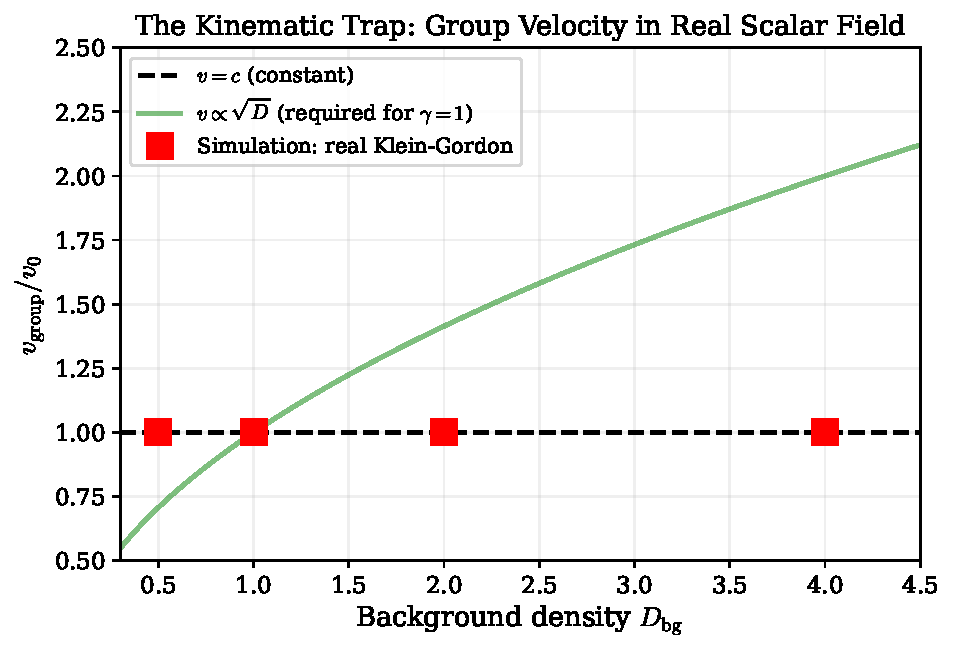
\includegraphics[width=0.7\columnwidth]{fig1_kinematic_trap.pdf}
    \caption{The kinematic trap. Group velocity of a wave packet in a Klein-Gordon field vs.\ background density $D_{\mathrm{bg}}$. The velocity is constant (red squares), confirming Eq.~(\ref{eq:eikonal}). The green curve shows the density dependence needed for $\gamma = 1$.}
    \label{fig:kinematic_trap}
\end{figure}

Since the coordinate speed of light cannot vary with the background, the only deflection contribution comes from time dilation:
\begin{equation}
    \delta\theta_{\mathrm{scalar}} = \frac{2GM}{bc^2}\,,
\end{equation}
giving $\gamma = 0$. This holds for \emph{any} potential $V(D)$: the characteristic surfaces of~(\ref{eq:general_kg}) are determined by the principal symbol (the D'Alembertian), not by $V$. Escaping this constraint requires either modifying the kinetic term, as in scalar-tensor theories~\cite{brans_1961}, or reinterpreting the field in a formulation where the propagation speed emerges dynamically.


% ====================================================================
\section{The Madelung Superfluid Formulation}
\label{sec:madelung}
% ====================================================================

\subsection{The logarithmic superfluid}

We model the vacuum as a complex order parameter $\psi(x,t)$ evolving under~\cite{zloshchastiev_2023,zloshchastiev_2020}:
\begin{equation}
    \Box\psi + \mu^2\psi - b\,\psi\,\ln\!\left(\frac{|\psi|^2}{\rho_0}\right) = 0\,.
\label{eq:log_kg}
\end{equation}
The logarithmic nonlinearity produces Gaussian-localized solitons (``Gaussons'')~\cite{bialynicki_birula_1979,avdeenkov_2011} and preserves the Landau roton-maxon spectrum~\cite{zloshchastiev_2012}.

\subsection{The Madelung decomposition}

Applying $\psi = \sqrt{\rho}\,e^{iS/\hbar_{\mathrm{eff}}}$ and separating real and imaginary parts yields two coupled equations:

\emph{Continuity} (conservation of vacuum flux):
\begin{equation}
    \partial_\mu(\rho\,\partial^\mu S) = 0\,.
\label{eq:continuity}
\end{equation}

\emph{Hamilton-Jacobi} (relativistic phase dynamics):
\begin{equation}
    \frac{1}{\hbar_{\mathrm{eff}}^2}\,\partial_\mu S\,\partial^\mu S = \mu^2 - b\,\ln\!\left(\frac{\rho}{\rho_0}\right) + \frac{\Box\sqrt{\rho}}{\sqrt{\rho}}\,.
\label{eq:hj}
\end{equation}
The last term is the quantum potential (Bohm potential), negligible in the macroscopic limit. The fluid four-velocity is $u_\mu = \partial_\mu S/m_{\mathrm{eff}}$, irrotational by construction except at topological defects (vortices).

The crucial point is that Eq.~(\ref{eq:hj}), unlike a wave equation, couples the phase gradient $\partial_\mu S$ to the density $\rho$ through a constraint that depends on the local thermodynamic state. This coupling produces a density-dependent sound speed, as we now show.


% ====================================================================
\section{Relativistic Sound Speed from the Logarithmic Equation of State}
\label{sec:sound_speed}
% ====================================================================

For a relativistic scalar field with Lagrangian density $\mathcal{L} = \rho X - V(\rho)$ where $X \equiv \partial_\mu S\,\partial^\mu S$ and $\rho = |\psi|^2$, the Hamilton-Jacobi equation in the macroscopic limit reads $X = V'(\rho)$, which allows the density to be integrated out in favor of $X$. The resulting effective Lagrangian $\mathcal{L}_{\mathrm{eff}}(X) = \rho(X)\,X - V(\rho(X))$ is of k-essence type, with pressure $p = \mathcal{L}_{\mathrm{eff}}$ and energy density $\epsilon = 2X\,\mathcal{L}'_{\mathrm{eff}} - \mathcal{L}_{\mathrm{eff}}$~\cite{babichev_mukhanov_vikman_2008}. Using the Barcel\'{o}-Liberati-Visser definition $c_s^2 = dp/d\epsilon$ for relativistic barotropic fluids~\cite{barcelo_2005}, one finds
\begin{equation}
    c_s^2 = \frac{\rho_0\,V''(\rho_0)}{\rho_0\,V''(\rho_0) + 2\,V'(\rho_0)}\,.
\label{eq:cs_general}
\end{equation}
As a check, the radiation-gas potential $V(\rho) = \tfrac{1}{2}g\rho^2$ gives $V' = g\rho$, $V'' = g$, $\rho V'' = g\rho = V'$, and Eq.~(\ref{eq:cs_general}) recovers the standard result $c_s^2 = 1/3$.

For the logarithmic potential $V(\rho) = -b\,\rho\,\ln(\rho/\rho_c)$, where the minus sign reflects the attractive (self-binding) interaction in Eq.~(\ref{eq:log_kg}):
\begin{equation}
    V' = -b\!\left[\ln\!\left(\frac{\rho}{\rho_c}\right) + 1\right]\!,\quad V'' = -\frac{b}{\rho}\,,\quad \rho_0 V'' = -b\,.
\end{equation}
Substituting (the minus signs cancel in the ratio):
\begin{equation}
    \boxed{\;c_s^2 = \frac{1}{2\ln(\bar{\rho}/\rho_c) + 3}\;}
\label{eq:cs_log}
\end{equation}
The coupling $b$ cancels, and $c_s$ depends on the local vacuum density $\bar{\rho}$ through the logarithm. Normalizing so that $c_s = c$ at the background density $\rho_\infty$ fixes $\rho_c = e\,\rho_\infty$.

This density dependence is a relativistic effect. In the non-relativistic logarithmic Schr\"{o}dinger equation, the denominator of~(\ref{eq:cs_general}) is dominated by $|V'(\rho_0)| \approx m_{\mathrm{eff}}c^2 \gg |\rho_0 V''|$, yielding $c_s^2 \approx |\rho_0 V''|/(2m_{\mathrm{eff}}c^2) \propto b/(m_{\mathrm{eff}}c^2)$, independent of density~\cite{avdeenkov_2011}. In the relativistic regime, $V'$ and $\rho_0 V''$ are comparable, and the density dependence survives (Fig.~\ref{fig:sound_speed}). Equation~(\ref{eq:cs_log}) also reveals a hard minimum density: at $\bar{\rho} = \rho_c\,e^{-3/2}$ the sound speed diverges, and below this threshold $c_s^2 < 0$, signaling breakdown of the hydrodynamic description.

\begin{figure}[H]
    \centering
    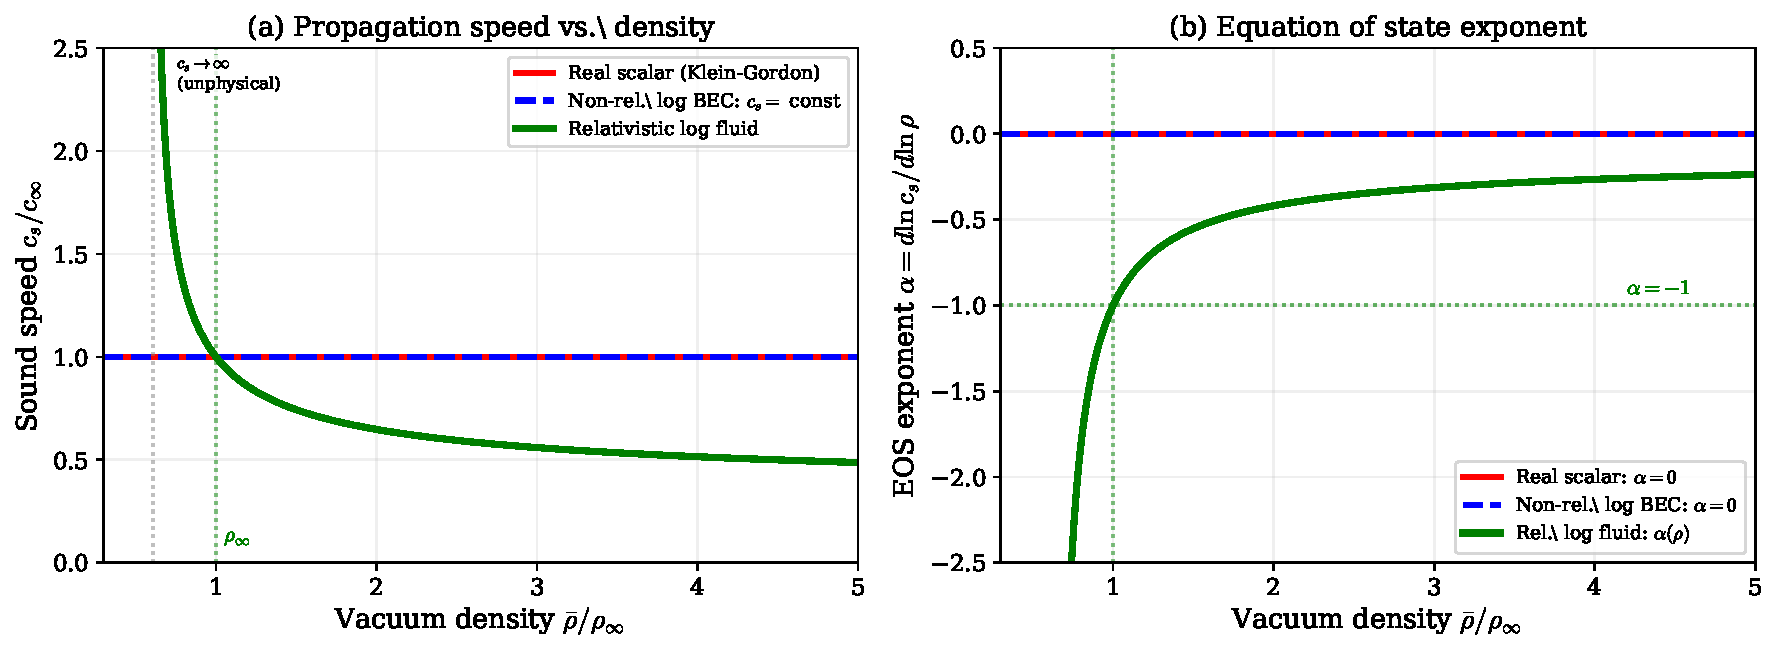
\includegraphics[width=\columnwidth]{fig2_sound_speed.pdf}
    \caption{(a)~Sound speed vs.\ density. The relativistic logarithmic fluid (green) has density-dependent $c_s$, while the real scalar KG and non-relativistic BEC give constant propagation speed. A singularity at $\bar{\rho}/\rho_c = e^{-3/2} \approx 0.22$ marks the minimum physical density. (b)~The equation of state exponent $\alpha = d\ln c_s/d\ln\rho$, crossing $\alpha = -1$ at $\bar{\rho} = \rho_\infty$.}
    \label{fig:sound_speed}
\end{figure}

The equation of state exponent, which controls the PPN structure, is:
\begin{equation}
    \alpha \equiv \frac{d\ln c_s}{d\ln\rho} = -\frac{1}{2\ln(\bar{\rho}/\rho_c) + 3}\,.
\label{eq:alpha}
\end{equation}
At the cosmological background $\bar{\rho} = \rho_\infty$ (where $\ln(\rho_\infty/\rho_c) = -1$): $\alpha = -1$.


% ====================================================================
\section{The Static Acoustic Metric and Its Limitations}
\label{sec:static}
% ====================================================================

\subsection{PPN parameter from the static metric}

For a static irrotational fluid with density $\bar{\rho}(x)$ and sound speed $c_s(x)$, the acoustic metric is~\cite{barcelo_2005,unruh_1981}:
\begin{equation}
    g_{tt} = -\bar{\rho}\,c_s\,,\qquad g_{ij} = \frac{\bar{\rho}}{c_s}\,\delta_{ij}\,.
\label{eq:static_metric}
\end{equation}
With $c_s \propto \bar{\rho}^{\,\alpha}$, a small density perturbation $\bar{\rho} = \rho_\infty(1+\epsilon)$ gives:
\begin{align}
    \frac{\delta g_{tt}}{g_{tt}} &= (1+\alpha)\,\epsilon\,,\label{eq:dgtt}\\
    \frac{\delta g_{rr}}{g_{rr}} &= (1-\alpha)\,\epsilon\,.\label{eq:dgrr}
\end{align}
Identifying $\Phi/c^2$ from the temporal component and reading off the spatial component:
\begin{equation}
    \boxed{\;\gamma_{\mathrm{static}} = \frac{1-\alpha}{1+\alpha}\;}
\label{eq:gamma_static}
\end{equation}
This is the PPN parameter for any static barotropic acoustic metric with equation of state exponent $\alpha$ (Fig.~\ref{fig:static_gamma}).

\begin{figure}[H]
    \centering
    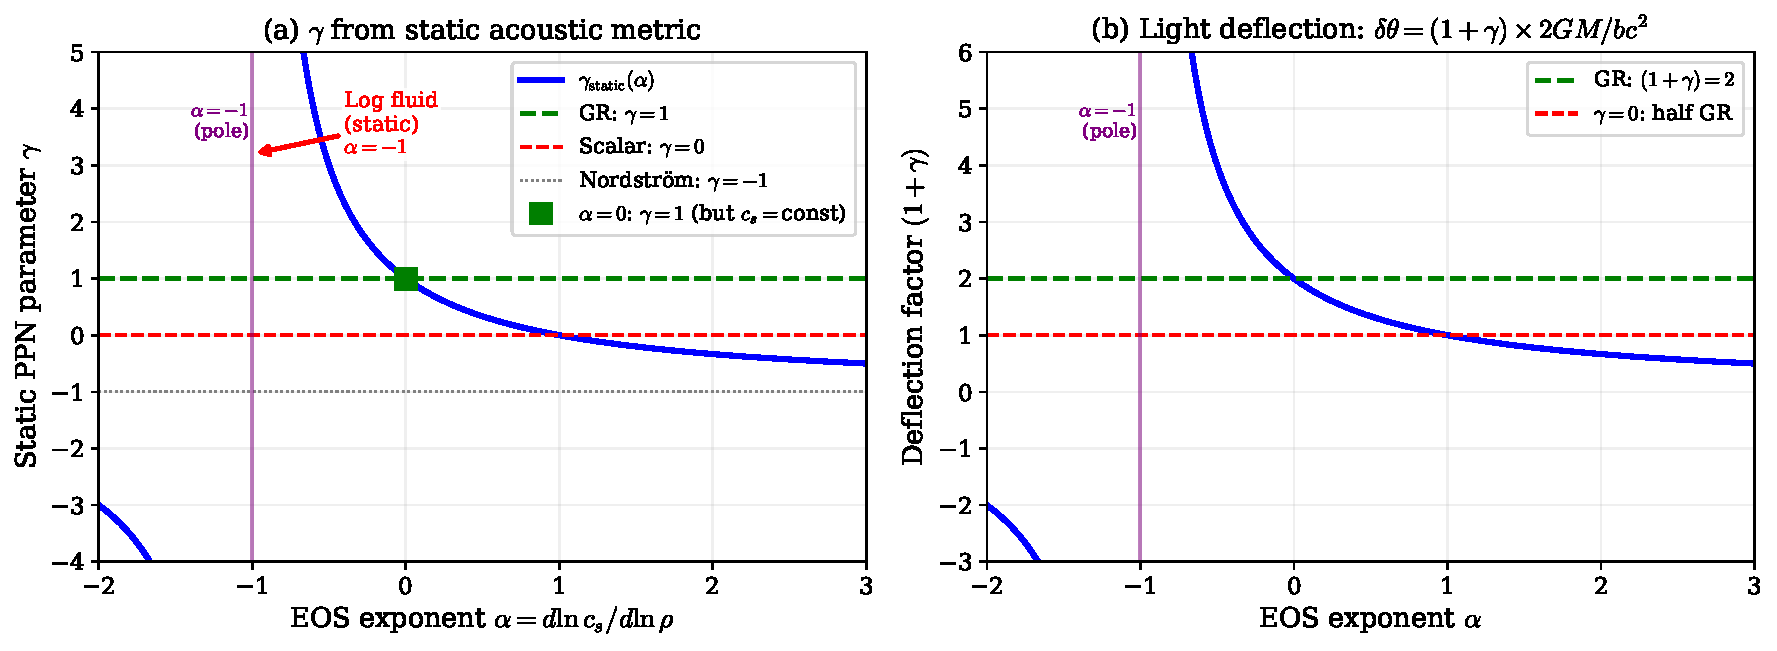
\includegraphics[width=\columnwidth]{fig3_static_gamma.pdf}
    \caption{(a)~Static PPN parameter $\gamma(\alpha) = (1-\alpha)/(1+\alpha)$. The logarithmic fluid at $\bar{\rho} = \rho_\infty$ has $\alpha = -1$, a pole of $\gamma_{\mathrm{static}}$: the static acoustic metric is ill-defined. GR's $\gamma = 1$ is attained at $\alpha = 0$, but this corresponds to density-independent $c_s$, which produces zero refractive deflection. (b)~The same pathology in the deflection factor $(1+\gamma)$.}
    \label{fig:static_gamma}
\end{figure}

\subsection{The static acoustic metric is pathological}

Equation~(\ref{eq:gamma_static}) reveals a fundamental obstruction. For the logarithmic equation of state at the background density, $\alpha = -1$, and the denominator of $\gamma_{\mathrm{static}}$ vanishes:
\begin{equation}
    \gamma_{\mathrm{static}} \to \infty \quad\text{at}\quad \alpha = -1\,.
\label{eq:gamma_pathology}
\end{equation}
The static acoustic metric does not merely give the wrong numerical value of $\gamma$; the spatial metric perturbation diverges relative to the temporal one, and no finite weak-field expansion around the static background is possible. Physically, the pole signals that the static configuration is not a stable background for perturbations: an arbitrarily small density gradient produces an arbitrarily large metric response.

This is, at a deeper level, a consequence of conformal invariance. For a static fluid with no flow, the acoustic metric~(\ref{eq:static_metric}) is conformally flat: $g_{\mu\nu} \propto (\bar{\rho}/c_s)\,\eta_{\mu\nu}^{(c_s)}$. Null geodesics are insensitive to the conformal factor, so light follows paths determined only by $c_s(x)$. Moreover, the PPN value $\gamma = 1$ is attained in Eq.~(\ref{eq:gamma_static}) only at $\alpha = 0$ (constant $c_s$), which produces no refractive deflection. The static acoustic metric therefore presents a twofold obstruction: the logarithmic model sits at the pole $\alpha = -1$, and even the regular point $\alpha = 0$ would give vanishing deflection. Any consistent treatment must therefore regularize the divergence by introducing additional dynamical content beyond the static density channel; this is the role of the Painlev\'{e}-Gullstrand flow developed in Sec.~\ref{sec:flowing}.


% ====================================================================
\section{The Flowing Acoustic Metric and the Path to \texorpdfstring{$\gamma = 1$}{gamma = 1}}
\label{sec:flowing}
% ====================================================================

\subsection{The Painlev\'{e}-Gullstrand structure}
The static metric exhausts only one of the two degrees of freedom provided by the Madelung decomposition. The second---the macroscopic flow velocity $\mathbf{v} = \nabla S/m_{\mathrm{eff}}$---contributes off-diagonal terms. For a spherically symmetric radial inflow $v(r)$ in a fluid with $\bar{\rho}/c_s \approx \text{const}$ and $c_s \approx c$, the acoustic metric takes the Painlev\'{e}-Gullstrand form~\cite{unruh_1981,visser_1998,volovik_2003}:
\begin{equation}
    ds^2 = -c^2 dt^2 + \big(dr + v(r)\,dt\big)^2 + r^2\,d\Omega^2\,.
\label{eq:pg_metric}
\end{equation}
If the flow velocity satisfies the free-fall profile:
\begin{equation}
    v(r) = \sqrt{\frac{2G_{\mathrm{eff}}M}{r}}\,,
\label{eq:pg_velocity}
\end{equation}
then the standard coordinate transformation $dt_s = dt - v\,dr/(c^2 - v^2)$ converts~(\ref{eq:pg_metric}) to the Schwarzschild metric:
\begin{equation}
    ds^2 = -\!\left(1 - \frac{2G_{\mathrm{eff}}M}{rc^2}\right)c^2 dt_s^2 + \frac{dr^2}{1 - 2G_{\mathrm{eff}}M/(rc^2)} + r^2 d\Omega^2\,,
\end{equation}
which gives $\gamma = 1$ exactly. The off-diagonal flow term breaks the conformal flatness of the static metric, introducing genuine spatial curvature through the $g_{rr} = (1 - v^2/c^2)^{-1}$ factor. That this specific velocity profile is not imposed by fiat but follows from a Bernoulli self-consistency condition is established in Sec.~\ref{par:bernoulli}.
The physical mechanism is frame-dragging by the inflowing vacuum: light propagating against the current is slowed (increased effective refractive index), while the spatial geometry is distorted by the kinetic energy of the flow. Both effects contribute to the deflection, and their combined weight gives the full GR value.

\subsection{Self-consistency test: Bondi accretion}

The Painlev\'{e}-Gullstrand argument assumes $v(r) = \sqrt{2G_{\mathrm{eff}}M/r} \propto r^{-1/2}$. We now ask: does this profile emerge self-consistently from the fluid equations with the logarithmic equation of state?

For steady-state spherical accretion, the continuity equation~(\ref{eq:continuity}) gives $4\pi r^2 \bar{\rho}\,v = \dot{M} = \text{const}$. If $\bar{\rho}$ is approximately constant (required for the Painlev\'{e}-Gullstrand form), then:
\begin{equation}
    v(r) \propto \frac{1}{r^2}\qquad\text{(continuity with $\bar{\rho} \approx \text{const}$)}\,.
\label{eq:bondi_scaling}
\end{equation}
This is incompatible with the required $v \propto r^{-1/2}$. The discrepancy grows as $(r_s/r)^{3/2}$, where $r_s = GM/(2c^2)$ is the sonic radius.

We verify this by solving the full Bondi accretion equations~\cite{bondi_1952}:
\begin{equation}
    \frac{dv}{dr} = \frac{v(2c_s^2/r - GM/r^2)}{v^2 - c_s^2}
\label{eq:bondi}
\end{equation}
with $c_s^2(\bar{\rho})$ given by Eq.~(\ref{eq:cs_log}) and $\bar{\rho}$ from continuity. The solution, passing through the sonic point ($v = c_s$ at $r = r_s$), is shown in Fig.~\ref{fig:bondi}.

\begin{figure}[H]
    \centering
    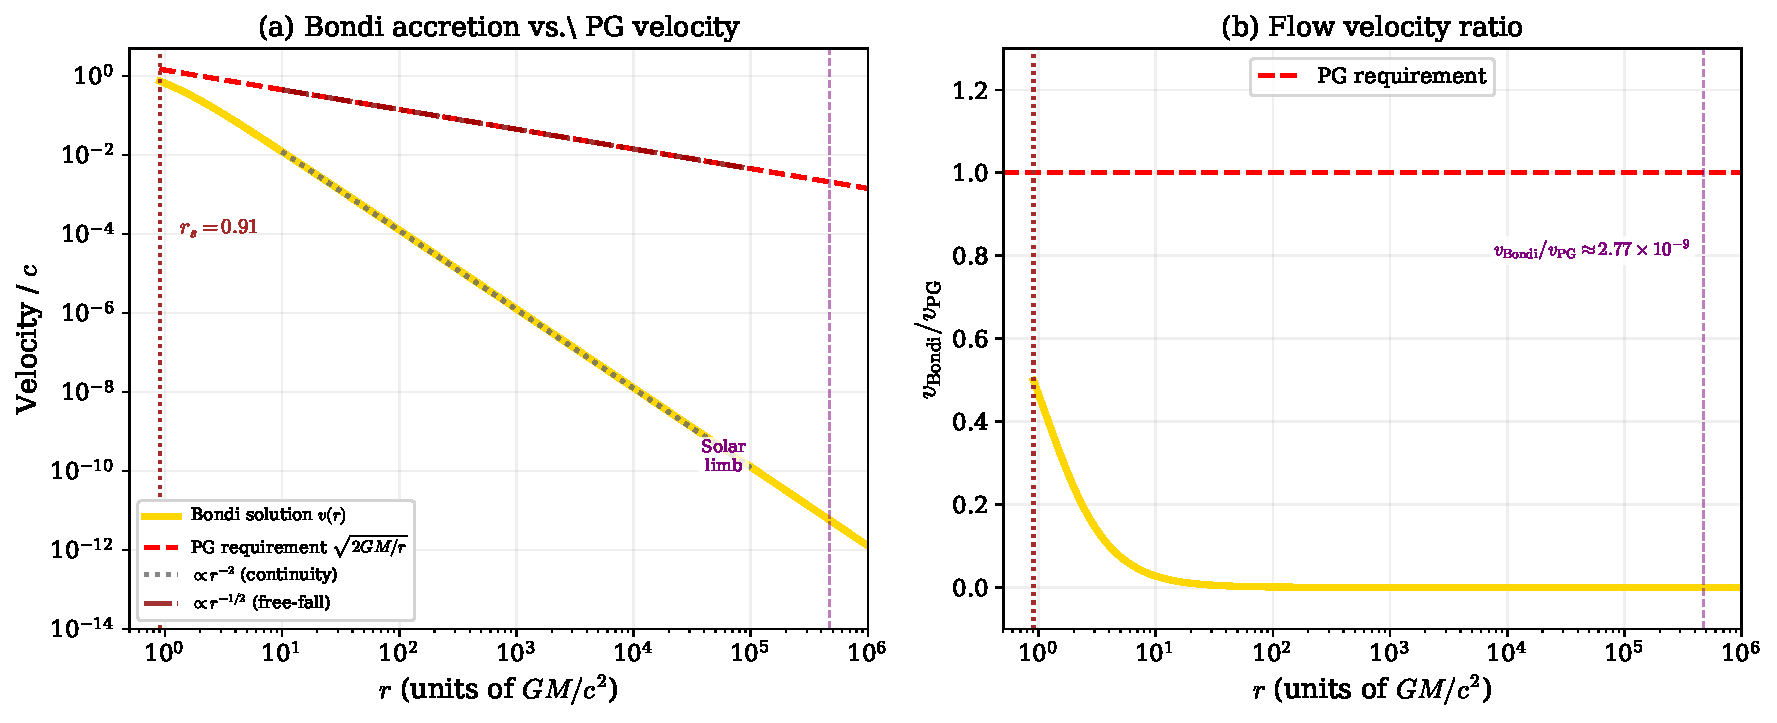
\includegraphics[width=\columnwidth]{fig4_bondi_vs_pg.pdf}
    \caption{(a)~Bondi accretion velocity (solid gold) vs.\ the Painlev\'{e}-Gullstrand requirement $v = \sqrt{2GM/r}$ (dashed red). In the subsonic far field, $v_{\mathrm{Bondi}} \propto r^{-2}$, falling far below the $r^{-1/2}$ profile. (b)~Ratio $v_{\mathrm{Bondi}}/v_{\mathrm{PG}}$. At the solar limb ($r \sim 5\times 10^5\,r_s$), the ratio is $\approx 2.8\times 10^{-9}$.}
    \label{fig:bondi}
\end{figure}

This establishes that single-soliton Bondi accretion cannot produce the PG profile required by the acoustic-metric consistency argument. The resolution is that the PG profile must arise from collective, many-soliton dynamics, not from single-source accretion—a point we return to in Sec.~\ref{par:collective_flow}.


% ====================================================================
\section{Discussion}
\label{sec:discussion}
% ====================================================================
\subsection{The circularity objection}

A natural objection: by placing $c$ in the D'Alembertian of Eq.~(\ref{eq:log_kg}), we assumed Lorentz invariance. Is $\gamma = 1$ then circular?

No. The D'Alembertian alone guarantees only that the
asymptotic propagation speed is $c$. As shown in
Sec.~\ref{sec:kinematic_trap}, the real scalar equation
$\Box D + V'(D) = 0$ also contains $c$ in its
D'Alembertian, yet gives $v = c = \mathrm{const}$
regardless of background, yielding $\gamma = 0$.
Lorentz invariance is necessary but not sufficient
for $\gamma = 1$.

What promotes $\gamma$ from 0 to 1 is the combination of three distinct structural features, none of which is present in the real-scalar theory:
\begin{enumerate}
\item \emph{The Madelung decomposition} promotes the field content from one real degree of freedom ($D$) to two real degrees of freedom (density $\rho$ and phase $S$), breaking the rigidity of the principal symbol.
\item \emph{The logarithmic nonlinearity}, in the \emph{relativistic} regime, produces a density-dependent sound speed with $\alpha = -1$ at the background (Eq.~\ref{eq:alpha}).
\item \emph{The Painlev\'{e}-Gullstrand flow} provides a second dynamical channel (the macroscopic flow velocity) that regularizes the static-metric divergence at $\alpha = -1$ and delivers $\gamma = 1$ for any barotropic equation of state.
\end{enumerate}
Each ingredient is individually insufficient: the real-scalar KG with the same D'Alembertian gives $\gamma = 0$; the Madelung decomposition alone in the non-relativistic limit gives $\alpha = 0$ and thus no refractive bending; the static acoustic metric alone at $\alpha = -1$ is pathological. Lorentz invariance is the foundation; the complex field structure, the relativistic log nonlinearity, and the macroscopic flow together build the house.

\subsection{The logical chain}
\label{subsec:logchain}
Our results establish a clear logical chain:

\paragraph{The kinematic trap is absolute}
Any real scalar field equation with a D'Alembertian kinetic term gives $\gamma = 0$, regardless of the self-interaction potential (Sec.~\ref{sec:kinematic_trap}). This is a property of the equation's characteristic surfaces, not of any particular solution.

\paragraph{The Madelung formulation breaks the trap}
The complex field's Madelung decomposition introduces two degrees of freedom---density $\rho$ and flow velocity $\mathbf{v}$---that are hidden in the wave equation form. The relativistic logarithmic equation of state yields a density-dependent sound speed (Eq.~\ref{eq:cs_log}), which is the prerequisite for any refractive bending mechanism.

\paragraph{The static acoustic metric is pathological}
The PPN parameter of a static barotropic acoustic metric is $\gamma = (1-\alpha)/(1+\alpha)$ (Eq.~\ref{eq:gamma_static}). For the logarithmic equation of state at the background density, $\alpha = -1$, placing $\gamma_{\mathrm{static}}$ exactly at the pole. The static acoustic metric is mathematically ill-defined, not merely numerically wrong.

\paragraph{Background flow is necessary and regularizes the pathology}
The Painlev\'{e}-Gullstrand form of the flowing acoustic metric reproduces the Schwarzschild geometry and $\gamma = 1$ exactly, provided $v(r) = \sqrt{2G_{\mathrm{eff}}M/r}$ (Sec.~\ref{sec:flowing}). The off-diagonal flow term $-2v\,dr\,dt$ cannot be removed by a conformal rescaling and carries the full $\gamma = 1$ result for any barotropic equation of state, independent of $\alpha$. In this way the flow regularizes the divergence of the static case: the dynamical content that the static metric could not carry in the (pathological) density channel is transferred to the (well-defined) flow channel.

\paragraph{The PG flow is the only self-consistent solution}
In the superfluid vacuum framework, the gravitational potential is not externally specified---it \emph{is} the acoustic metric. This imposes a self-consistency requirement: the density perturbation $\epsilon = \delta\rho/\rho_0$ and flow velocity $v(r)$ must produce an acoustic metric whose effective Newtonian potential $\Phi_{\mathrm{eff}} = -\tfrac{1}{2}\delta g_{tt}/g_{tt}$ matches the potential that generated $\epsilon$ and $v$ in the first place.

For the static solution (Solution~A: $v = 0$, $\epsilon \neq 0$), the divergence of $\gamma_{\mathrm{static}}$ at $\alpha = -1$ means that no finite density perturbation $\epsilon$ produces a finite weak-field metric: the self-consistency equation admits no regular solution in this channel.

For the flowing solution (Solution~B: $v = \sqrt{2G_{\mathrm{eff}}M/r}$, $\rho \approx \rho_0$), the Bernoulli equation gives $\tfrac{1}{2}v^2 + \Phi_{\mathrm{eff}} = 0$ at leading order, and the acoustic metric in Schwarzschild coordinates gives $g_{tt} \approx -(1 - 2U)$, $g_{rr} \approx (1 + 2U)$, yielding $\Phi_{\mathrm{eff}} = -U$ and $\gamma = 1$. The Bernoulli relation $v^2 = 2U$ then closes the loop: $\Phi_{\mathrm{eff}}$ produces the flow that produces $\Phi_{\mathrm{eff}}$. This solution \emph{is} self-consistent for any barotropic equation of state, because the Painlev\'{e}-Gullstrand acoustic metric is identically the Schwarzschild metric regardless of the specific form of $c_s(\rho)$.

\paragraph{Independent confirmation from Bernoulli dynamics}
\label{par:bernoulli}
The Painlev\'{e}-Gullstrand requirement can be derived 
independently from the Bernoulli relation of the logarithmic fluid. Linearizing the Hamilton-Jacobi equation~(\ref{eq:hj}) about the background with $|\mathbf{v}| \ll c$ and using $V'(\rho_0) = -b[\ln(\rho_0/\rho_c) + 1]$, one obtains $\ln(\rho/\rho_\infty) = +(m_{\mathrm{eff}}^2/b\hbar_{\mathrm{eff}}^2)\,|\mathbf{v}|^2$ to leading order. With the convention $\delta\rho \equiv \rho_\infty - \rho > 0$ for the depletion in a gravitational well, this gives $\delta\rho/\rho_\infty \propto v^2$ in the weak-field limit. Since Newtonian gravity requires a density depletion $\delta\rho \propto 1/r$ (from the Poisson equation combined with the framework's identification $\Phi \propto -\delta\rho$), the flow velocity must satisfy $v^2 \propto 1/r$, recovering the Painlev\'{e}-Gullstrand profile $v = \sqrt{2G_{\mathrm{eff}}M/r}$ from a purely hydrodynamic argument. This provides a second, independent derivation of the PG condition, complementing the acoustic metric self-consistency argument above.

\paragraph{The continuity constraint}
The radially inward PG flow $\mathbf{v} = -\sqrt{2GM/r}\,\hat{\mathbf{r}}$ has $\nabla \cdot \mathbf{v} = -\tfrac{3}{2}\sqrt{2GM}\,r^{-3/2} \neq 0$, corresponding to condensate accumulation $\partial\rho/\partial t = -\rho_0 \nabla \cdot \mathbf{v} > 0$. The accumulation rate is small: at the solar limb, $|\nabla \cdot \mathbf{v}|^{-1} \sim 10^3$~s, but this timescale applies to fractional changes $\delta\rho/\rho_0 \sim U \sim 10^{-6}$, so the absolute density change per observation epoch is negligible. The PG flow is a valid quasi-steady approximation on all timescales short compared to the gravitational collapse time. A fully steady-state treatment requires a mechanism that redirects the inflowing condensate without local accumulation; candidate mechanisms include two-fluid counterflow, vortex-core absorption, and geometric redirection into non-radial outflow. The choice of mechanism is deferred to future work.

\paragraph{Single-particle vs.\ collective flow}
\label{par:collective_flow}
The Bondi accretion solution for the logarithmic equation of state does not produce the required velocity profile in the far field. Continuity enforces $v \propto r^{-2}$ for nearly-incompressible steady flow, while $\gamma = 1$ requires $v \propto r^{-1/2}$. This discrepancy applies to single-soliton configurations. However, the self-consistency argument above does not depend on the single-particle velocity field. The PG flow must arise as a \emph{collective} effect of $N \sim M/m_{\mathrm{particle}}$ solitons: individual particles contribute microscopic density perturbations that sum to the macroscopic potential $\Phi = -GM/r$, and the resulting vacuum inflow adjusts to maintain self-consistency of the acoustic metric. In this picture, the Bondi calculation describes the flow around a single vortex core (irrelevant at astrophysical distances), while the PG flow describes the macroscopic vacuum response to the collective mass distribution. The relationship between the microscopic and macroscopic descriptions---analogous to the Feynman-Onsager relation in rotating superfluids---remains an open problem.

Two open problems remain. First, deriving the macroscopic PG flow from the microscopic soliton dynamics: showing that a collection of $N$ vortex-Gaussons in the logarithmic condensate produces a collective vacuum inflow $v = \sqrt{2GM/r}$ as a mean-field effect, analogous to how a lattice of quantized vortices in superfluid helium produces solid-body rotation~\cite{volovik_2003}. Second, establishing the steady-state mechanism: identifying whether the two-fluid counterflow (superfluid infall balanced by normal-component outflow) or vortex-core absorption provides the sink term required for continuity. The first problem is amenable to a Thomas-Fermi mean-field calculation; the second requires understanding the quantum depletion of the condensate in the presence of topological defects.


\subsection{Relation to prior work}

The superfluid vacuum program of Zloshchastiev~\cite{zloshchastiev_2023,zloshchastiev_2020,zloshchastiev_2011} derives emergent spacetime metrics from the logarithmic condensate but does not compute PPN parameters explicitly. The analogue gravity program of Barcel\'{o}, Liberati, and Visser~\cite{barcelo_2005,barcelo_2011} proves that fluid perturbations propagate on acoustic metrics but does not construct specific models matching solar system tests. The present work connects these programs by deriving the explicit PPN constraints and identifying the gap between the static and flowing acoustic metrics.

The flowing acoustic metric's equivalence to the Painlev\'{e}-Gullstrand form of Schwarzschild was noted by Unruh~\cite{unruh_1981} and developed extensively by Visser~\cite{visser_1998} and Volovik~\cite{volovik_2003}. Our contribution is to test this identification against self-consistent fluid dynamics, revealing that the velocity profile is not automatically produced.

\subsection{Limitations}

\paragraph{Conformal flatness and strong fields}
The acoustic metric~(\ref{eq:static_metric}) is
conformally flat ($g_{ij} \propto \delta_{ij}$).
General relativity admits nontrivial Weyl curvature. The present framework reproduces the weak-field PPN limit but cannot describe strong-field phenomena: binary pulsar orbital decay~\cite{taylor_1979}, black hole ringdown, or nonlinear gravitational wave dynamics. Whether extensions incorporating vorticity or background flow can access the strong-field regime is an open question.

\paragraph{The quantum potential}
The Bohm potential $Q = \Box\sqrt{\rho}/\sqrt{\rho}$
was neglected in the macroscopic limit. At the soliton coherence scale, $Q$ becomes
important and governs quantum-mechanical particle
behavior. A complete theory must show a smooth
transition between quantum and gravitational regimes
---analogous to the phonon-to-hydrodynamic crossover
in superfluid helium~\cite{volovik_2003}.

\subsection{Additional constraints}

The recovery of $\gamma = 1$ via the Painlev\'{e}-Gullstrand structure, if achieved, would automatically resolve the Shapiro time delay, since the PPN framework packages all weak-field solar system tests into the parameters $\{\gamma, \beta, \ldots\}$~\cite{will_2014}. The GW170817 constraint ($|c_{\mathrm{gw}} - c|/c < 10^{-15}$~\cite{abbott_2017}) requires that the asymptotic sound speed equal $c$ exactly, fixing a combination of the equation of state parameters. The second PPN parameter $\beta$, controlling perihelion precession, requires a higher-order post-Newtonian expansion beyond this work's scope.


% ====================================================================
\section{Conclusion}
\label{sec:conclusion}
% ====================================================================

We have shown that the failure of scalar gravity to produce the observed light bending is a property of the wave equation representation, not of scalar fields per se. The Madelung decomposition of a relativistic logarithmic superfluid introduces two degrees of freedom---a density-dependent sound speed and a macroscopic flow velocity---that together provide the structural ingredients needed for $\gamma = 1$.

The static acoustic metric of the logarithmic superfluid is mathematically pathological: the equation of state exponent $\alpha = -1$ at the background density places the static PPN parameter $\gamma_{\mathrm{static}} = (1-\alpha)/(1+\alpha)$ exactly at the pole. No finite weak-field expansion around the static background exists. By contrast, the Painlev\'{e}-Gullstrand flow $v = \sqrt{2G_{\mathrm{eff}}M/r}$ regularizes this pathology: the resulting acoustic metric is identically Schwarzschild in Painlev\'{e}-Gullstrand coordinates, and $\gamma = 1$ follows for \emph{any} barotropic equation of state. This selects the flowing solution as the unique physically admissible weak-field configuration.

The Bondi accretion calculation shows that a single spherically symmetric source does not produce the PG profile: far from the sonic radius the flow decays as $r^{-2}$, falling nearly nine orders of magnitude below the $r^{-1/2}$ requirement at the solar limb. The remaining open problems are therefore to derive the macroscopic PG flow as a collective mean-field effect of the microscopic soliton dynamics---analogous to the Feynman-Onsager relation in rotating superfluids---and to identify the steady-state mechanism (two-fluid counterflow or vortex-core absorption) that resolves the continuity constraint. Both are amenable to analytical treatment and form the subject of forthcoming work.

% ====================================================================
\section*{Acknowledgments}
% ====================================================================

The author thanks K.~G.~Zloshchastiev for foundational work on the logarithmic superfluid vacuum and C.~Barcel\'{o}, S.~Liberati, and M.~Visser for the acoustic metric framework. Claude (Anthropic) and Gemini (Google) were used as editorial and computational tools during manuscript preparation. All scientific content, equations, and interpretations are the author's own.


\begin{thebibliography}{25}

\bibitem{babichev_mukhanov_vikman_2008}
E.~Babichev, V.~Mukhanov, and A.~Vikman,
k-Essence, superluminal propagation, causality and emergent geometry,
JHEP \textbf{02}, 101 (2008).

\bibitem{will_2014}
C.~M.~Will,
\emph{Theory and Experiment in Gravitational Physics}, 2nd ed.\ (Cambridge, 2014).

\bibitem{bertotti_2003}
B.~Bertotti, L.~Iess, and P.~Tortora,
A test of general relativity using radio links with the Cassini spacecraft,
Nature \textbf{425}, 374 (2003).

\bibitem{nordstrom_1913}
G.~Nordstr\"{o}m,
Zur Theorie der Gravitation vom Standpunkt des Relativit\"{a}tsprinzips,
Ann.\ Phys.\ (Leipzig) \textbf{347}, 533 (1913).

\bibitem{einstein_1911}
A.~Einstein,
\"{U}ber den Einflu\ss{} der Schwerkraft auf die Ausbreitung des Lichtes,
Ann.\ Phys.\ (Leipzig) \textbf{340}, 898 (1911).

\bibitem{zloshchastiev_2023}
K.~G.~Zloshchastiev,
Derivation of emergent spacetime metric, gravitational potential and speed of light in superfluid vacuum theory,
Universe \textbf{9}, 234 (2023).

\bibitem{zloshchastiev_2020}
K.~G.~Zloshchastiev,
An alternative to dark matter and dark energy: Scale-dependent gravity in superfluid vacuum theory,
Universe \textbf{6}, 180 (2020).

\bibitem{zloshchastiev_2011}
K.~G.~Zloshchastiev,
Spontaneous symmetry breaking and mass generation as built-in phenomena in logarithmic nonlinear quantum theory,
Acta Phys.\ Polon.\ B \textbf{42}, 261 (2011).

\bibitem{zloshchastiev_2012}
K.~G.~Zloshchastiev,
Volume element structure and roton-maxon-phonon excitations in superfluid helium beyond the Gross-Pitaevskii approximation,
Eur.\ Phys.\ J.\ B \textbf{85}, 273 (2012).

\bibitem{bialynicki_birula_1979}
I.~Bia\l{}ynicki-Birula and J.~Mycielski,
Gaussons: Solitons of the logarithmic Schr\"{o}dinger equation,
Phys.\ Scr.\ \textbf{20}, 539 (1979).

\bibitem{avdeenkov_2011}
A.~V.~Avdeenkov and K.~G.~Zloshchastiev,
Quantum Bose liquids with logarithmic nonlinearity: Self-sustainability and emergence of spatial extent,
J.\ Phys.\ B \textbf{44}, 195303 (2011).

\bibitem{barcelo_2005}
C.~Barcel\'{o}, S.~Liberati, and M.~Visser,
Analogue gravity,
Living Rev.\ Rel.\ \textbf{8}, 12 (2005);
updated: \textbf{14}, 3 (2011).

\bibitem{barcelo_2011}
C.~Barcel\'{o}, S.~Liberati, and M.~Visser,
Analogue models for FRW cosmologies,
Class.\ Quant.\ Grav.\ \textbf{18}, 1137 (2001).

\bibitem{taylor_1979}
J.~H.~Taylor, L.~A.~Fowler, and P.~M.~McCulloch,
Measurements of general relativistic effects in the
binary pulsar PSR~1913+16,
Nature \textbf{277}, 437 (1979).

\bibitem{unruh_1981}
W.~G.~Unruh,
Experimental black-hole evaporation?,
Phys.\ Rev.\ Lett.\ \textbf{46}, 1351 (1981).

\bibitem{visser_1998}
M.~Visser,
Acoustic black holes: Horizons, ergospheres and Hawking radiation,
Class.\ Quant.\ Grav.\ \textbf{15}, 1767 (1998).

\bibitem{volovik_2003}
G.~E.~Volovik,
\emph{The Universe in a Helium Droplet} (Oxford, 2003).

\bibitem{bondi_1952}
H.~Bondi,
On spherically symmetrical accretion,
Mon.\ Not.\ Roy.\ Astron.\ Soc.\ \textbf{112}, 195 (1952).

\bibitem{abbott_2017}
B.~P.~Abbott \emph{et al.},
Gravitational waves and gamma-rays from a binary neutron star merger: GW170817 and GRB~170817A,
Astrophys.\ J.\ Lett.\ \textbf{848}, L13 (2017).

\bibitem{brans_1961}
C.~Brans and R.~H.~Dicke,
Mach's principle and a relativistic theory of gravitation,
Phys.\ Rev.\ \textbf{124}, 925 (1961).

\end{thebibliography}

\end{document}
